\documentclass{svproc}
\usepackage{newtxmath}
\usepackage{fontspec}
\setmainfont{Times New Roman}
\usepackage{microtype}
\setlength{\emergencystretch}{2em}
\usepackage{url}
\def\UrlFont{\rmfamily}
\usepackage{graphicx,booktabs,amsmath,placeins}
\usepackage[hidelinks]{hyperref}
\hypersetup{pdfauthor={},pdftitle={Validity Is Not Utility},pdfsubject={Anonymous IntelliSys 2027 research draft}}
\begin{document}
\mainmatter
\title{Validity Is Not Utility: A Paired Audit of Constraint Repair and Class Coverage in Synthetic Tabular Data}
\titlerunning{Constraint Repair and Class Coverage in Synthetic Data}
\author{}\authorrunning{}\institute{}
\maketitle
\begin{abstract}
Synthetic tabular data can satisfy explicit record constraints while failing to preserve predictive relationships. This distinction matters when intelligent data pipelines approve releases using validity scores alone. We ask whether eliminating feature-constraint violations preserves downstream minority-class utility, and whether feature-only rejection changes class coverage. A locally frozen protocol compares independent marginals, a joint Gaussian-rank copula, and a label-conditional copula on Adult, Bank Marketing, and red Wine Quality. Five stratified folds pair four processing methods on identical candidate pools: unchanged release, deterministic projection, rejection, and training-prevalence quota rejection. The study executes 210 predictive evaluations, including real-training and empirical-bootstrap references, and retains 195 generated releases. All three processing methods eliminate the tested violations. Nevertheless, projection reduces Adult minority-class F1 in every fold for both copula generators; the label-conditional mean falls from 66.8\% to 65.4\%. Feature-only rejection shifts class prevalence because validity acceptance differs by label: Adult conditional-pool acceptance averages 22.2\% for negatives and 17.5\% for positives. Quotas restore training prevalence but require 5.75 candidates per released row and do not recover the raw-release F1. Wine projection leaves thresholded F1 unchanged for the conditional generator. These results support separate validity, class-coverage, utility, and candidate-budget checks rather than a single synthetic-data approval score. The contribution is a reproducible diagnostic audit, not a new generator or a privacy guarantee.
\keywords{Synthetic tabular data, Constraint repair, Trustworthy AI, Class imbalance, Data quality}
\end{abstract}

\section{Introduction}
A valid synthetic record is not necessarily a useful training example. An education category may match its numeric code while its association with income is weakened. A record can correctly encode whether a customer was contacted before, yet a filtering rule can remove a disproportionate share of customers who subscribe. A pipeline that checks only whether generated rows satisfy business or scientific constraints can therefore approve a release with altered predictive behavior.

This paper studies the release decision after generation. The central question is: \emph{when a synthetic-data pipeline repairs invalid rows or discards them, which properties of the released data are actually preserved?} We distinguish feature validity, target-class coverage, downstream predictive utility, marginal fidelity, and candidate requirements. These are operationally different quantities. A repair can improve one without improving the others.

Constraint-aware generation is established. Stoian et al. integrate a constraint layer into deep generative models and examine its use during training and inference \cite{stoian2024}. We do not propose projection, rejection, or class quotas as new algorithms. Instead, we contribute a controlled comparison in which all postprocessing methods see the same generated candidates, release the same number of rows when feasible, and train the same downstream learner. The purpose is to expose the consequences of a validity intervention independently of variation between candidate draws.

The study is relevant to trustworthy intelligent data systems because automated release gates turn quality checks into approval decisions. Such a gate needs evidence about its intended downstream task. Classical generators provide a transparent diagnostic setting before extending the evaluation to more expensive neural synthesis. This is a bounded empirical investigation; it neither evaluates an LLM nor establishes a mathematical lower bound on modern generators.

Three questions guide the evaluation. \textbf{RQ1:} Does eliminating feature-constraint violations improve held-out real-data minority-class F1? \textbf{RQ2:} Can feature-only rejection change target prevalence, and does enforcing class quotas recover utility? \textbf{RQ3:} What tradeoffs arise in marginal fidelity, candidate examinations, and exact training-row replication relative to empirical resampling?

We execute a new five-fold study on three public datasets with three generators and four processing methods. The contribution comprises an explicit paired evaluation contract, an analytic explanation of class selection under rejection, and measured counterexamples to treating full validity as evidence of preserved utility. Source code, generated releases, split identities, predictions, and result tables are retained for reproduction. No estimated utility curve or previously reported experiment supplies a result in this paper.

\section{Related Work and Positioning}
Tabular generation must handle mixed types, multimodal variables, and imbalanced categories. CTGAN addresses these challenges using conditional adversarial generation \cite{xu2019}. Our label-conditional baseline is a simple rank-copula implementation, not CTGAN or a substitute benchmark for neural synthesis. We expose implementation choices such as category ordering and covariance shrinkage. Conclusions concern this evaluation contract and its tested generators; superiority over contemporary neural methods remains untested.

Constraint-aware synthesis provides a closer context. The constraint layer of Stoian et al. can ensure compliance and sometimes improve utility \cite{stoian2024}. That finding is compatible with our question: improvement is an empirical outcome, not a logical consequence of compliance. Our interventions are hand-specified, dataset-specific postprocessing rules. We compare changing a dependent field with retaining only valid candidates, and separately inspect how either choice affects rare positive labels.

Yang et al. advocate structured evaluation and model-free baselines rather than interpreting isolated metrics without a coherent objective \cite{yang2024}. We operationalize a narrow version of that concern: a feature check, a marginal-distance score, and a train-synthetic/test-real predictive score answer different questions. Whole-row bootstrap is included because it preserves empirical dependence while visibly copying training records. It is an informative utility reference and a poor privacy solution.

Our novelty claim is limited to this reproducible paired audit and its observed interactions between validity processing, class selection, and utility. We introduce no new architecture, privacy mechanism, selection-bias theorem, or universal enterprise-compliance score. The study replaces broad framework-level claims with directly measured outcomes on explicitly bounded tasks.

\section{Release Contract and Selection Mechanism}
\subsection{Paired Processing Methods}
Let a training set contain $n$ labeled rows $(x,y)$, and let a fitted generator produce a candidate sequence $S=(s_1,\ldots,s_{10n})$. A feature-only predicate $V(x)$ declares whether a row satisfies the selected rule. Every method shares this sequence and aims to release $n$ rows:
\begin{enumerate}
\item \textbf{Raw}: release the first $n$ candidates unchanged.
\item \textbf{Project}: apply the fixed repair map to those same first $n$ candidates; preserve each target label and every other field.
\item \textbf{Reject}: release the first $n$ candidates satisfying $V$.
\item \textbf{Quota}: scan valid candidates in order, also requiring $n_1=\operatorname{round}(n\hat p)$ positive and $n-n_1$ negative labels, where $\hat p$ is training prevalence.
\end{enumerate}
These are paired interventions on a generated pool, not independent replications. Projection changes values while retaining rows and labels; rejection changes which rows enter the release. Quota rejection additionally uses generated labels and real training prevalence. It is therefore not a label-blind filter. An exhausted pool is a failed complete release; invalid backfill is prohibited. All releases completed in this run.

We record the prefix length examined divided by $n$. This measures how much of the shared pool must be scanned. It is not wall-clock speed or a count of separately executed generator invocations: each pool is generated once in a batch, and its cost is shared across methods. The tenfold cap is prospective and finite; costs cannot be extrapolated to arbitrarily strict rules.

\subsection{Why a Feature-Only Rule Can Select Labels}
Write $p=P(Y=1)$ for candidate-pool prevalence and $a_y=P(V=1\mid Y=y)$ for class-conditional validity. Provided $P(V=1)>0$, ordinary conditioning gives
\begin{equation}
P(Y=1\mid V=1)=\frac{p a_1}{p a_1+(1-p)a_0}.\label{eq:selection}
\end{equation}
A rule does not have to read $Y$ to change its distribution. If feature validity and the label are associated, $a_1\ne a_0$, conditioning on validity selects labels indirectly. In a finite pool the identity holds exactly for the full set of valid rows. The first-$n$ prefix has additional sampling variation. We retain both quantities rather than presenting the identity as a fitted model.

Quotas fix the released target count up to rounding. They do not guarantee that conditional feature distributions match real training data, nor that a classifier learned from them performs well. Projection also lacks a utility guarantee: changing a field can change the predictor while row count and labels remain fixed.

\section{Data, Constraints, and Generators}
\subsection{Public Data and Targets}
Adult \cite{adult} uses the first 6,000 complete rows of \texttt{adult.data}, after omitting rows with missing values. The source file has 32,561 rows; this subset is a computational restriction, not a representative random sample of all Adult records. We do not use the provided \texttt{adult.test}. The target is income above 50,000 dollars; 1,499 analysis rows are positive.

Bank Marketing \cite{bank} uses the supplied \texttt{bank.csv} subset, with 4,521 rows and 521 positive subscription outcomes. It does not use the larger or additional bank files. Red Wine Quality \cite{wine} uses all 1,599 red-wine rows; quality at least seven defines 217 positives. The binary threshold was specified before evaluation. These tasks offer three small diagnostic cases, not comprehensive enterprise validation.

Table~\ref{tab:rules} specifies the complete intervention. Adult uses the documented education-category ordering, with codes one through sixteen. Bank checks the consistency of prior-contact count and the sentinel for no prior contact. Wine checks that total sulfur is at least free sulfur. No analysis row violates its selected rule, and no real rows are removed on the basis of that check. These limited checks do not imply complete record realism.

\begin{table}[!htbp]
\caption{Feature-only checks and deterministic repair fields.}\label{tab:rules}
\centering\small
\begin{tabular}{p{.12\textwidth}p{.43\textwidth}p{.31\textwidth}}\toprule
Data & Required relation & Projection \\\midrule
Adult & Education number equals category code & Replace education number \\
Bank & $\texttt{pdays}=-1$ iff $\texttt{previous}=0$; previous nonnegative & Set previous to zero if no prior contact, otherwise at least one \\
Wine & Total sulfur $\geq$ free sulfur & Raise total sulfur to free sulfur if needed \\\bottomrule
\end{tabular}
\end{table}
\FloatBarrier

\subsection{Transparent Baselines}
\textbf{Independent marginals} sample each feature and the target independently from its training empirical distribution. This deliberately weak baseline destroys dependence while preserving marginal support. It diagnoses whether a processing gain depends on an inadequate generator; it cannot establish competitive synthesis quality.

\textbf{Joint Gaussian-rank copula} encodes nominal categories using their alphabetical training-category order. For each column, midranks $r$ are transformed using $\Phi^{-1}((r-0.5)/n)$. The sample correlation matrix is shrunk as $0.95R+0.05I$, with numerical eigenvalue clipping at $10^{-8}$. Multivariate normal draws are mapped through $\Phi$ and an empirical inverse distribution. The target is a joint discrete column. No interpolation creates unseen numerical values.

\textbf{Label-conditional copula} fits a separate feature copula within each training class using the same transform and shrinkage. Synthetic labels are Bernoulli draws at training prevalence, followed by conditional feature generation. This preserves more label dependence by construction, but still imposes an arbitrary ordering on nominal features. It tests whether the main result survives beyond independent marginals.

\textbf{Empirical bootstrap} samples complete training rows with replacement to form an $n$-row release. It provides a dependence-preserving reference and an explicit copying comparator. A classifier trained on the unresampled real training partition is the separate real-training reference. Neither is an upper bound for every future model or release.

\section{Experimental Protocol}
\subsection{Splits, Predictors, and Metrics}
Five stratified folds use shuffle seed 2027. Every analysis row is held out once; each generator is fitted only on the remaining approximately 80\%. Adult training sets have 4,800 rows, Bank 3,616--3,617, and Wine 1,279--1,280. Dataset/fold-specific generator seeds and exact train/test row indices are retained. Each generator/fold produces one pool of $10n$ candidates. No test performance selects a generator, repair, hyperparameter, or classification threshold.

The downstream learner is class-balanced logistic regression with $C=1$, L-BFGS, and at most 1,000 iterations, implemented with scikit-learn \cite{sklearn}. Standardization and dense one-hot encoding are fitted on real training data and reused across that fold's releases; unknown categories are ignored. This assumes the original curator supplies preprocessing, rather than testing a release-only recipient pipeline. The probability threshold is fixed at 0.5. Scores and decisions on held-out real rows are retained.

Primary utility is positive-class F1. We also retain recall, balanced accuracy, average precision, and accuracy. Class coverage is measured by positive prevalence and its absolute difference from real training prevalence. Validity is the violation fraction. Marginal distance averages categorical total variation and numerical Wasserstein distance divided by training interquartile range, with range and unit fallbacks when necessary. This mixed score is descriptive, not a calibrated cross-domain quality scale.

Exact full-row training-match rate reports the fraction identical to any training record, including the target. It does not test membership inference, nearest-neighbor disclosure, linkage, or differential privacy. Zero matches do not establish safety. Bootstrap has 100\% exact matches by construction.

\subsection{Timing, Pairing, and Evidence Boundaries}
A local protocol was written before evaluation, specifying data, generators, rules, methods, budgets, folds, and metrics. It is not an external preregistration. The runner hashes protocol, source, raw archives, and itself before fitting. The protocol's description of split/environment fingerprinting was broader than implemented: deterministic split indices and environment versions were saved at run completion. This recording deviation does not change the splits or measured outcomes and is disclosed in the reproduction notes.

There are $3\times3\times4\times5=180$ generated-method evaluations, 15 bootstrap and 15 real-training references: 210 fits and 195 retained generated releases. Test folds are disjoint within each dataset, but training partitions overlap. Fold ranges and paired effects indicate within-dataset sensitivity, not independent population replications. We retain 2,000-resample paired-fold bootstrap stability intervals as conditional descriptions, not confirmatory confidence guarantees. No post-result tuning or selective rerun supplies the tables.

\section{Results}
\subsection{Validity and Utility Separate}
All 135 processed generator releases satisfy the tested constraint in every row. Their common 100\% validity does not imply common predictive performance. Table~\ref{tab:utility} reports mean F1 over five paired folds. Conditional raw releases have 79.4\%, 10.7\%, and 2.1\% violation rates on Adult, Bank, and Wine; projection removes these violations without changing labels.

On Adult, conditional projection reduces F1 from 66.8\% to 65.4\%, a paired mean change of $-1.38$ percentage points (pp). All five folds decrease, with effects from $-1.98$ to $-0.48$ pp. The conditional stability interval is $[-1.82,-0.92]$ pp. Joint-copula projection also decreases Adult F1 in all five folds, with mean $-2.59$ pp and range $[-3.99,-0.76]$. The negative result is not confined to independent marginals.

\begin{table}[!htbp]
\caption{Positive-class F1 (\%), mean of five folds on real test rows.}\label{tab:utility}
\centering\small
\begin{tabular}{llrrrr}\toprule
Data & Generator & Raw & Project & Reject & Quota \\\midrule
Adult & Marginals & 28.0 & 27.8 & 33.9 & 35.1 \\
Adult & Joint copula & 56.9 & 54.3 & 55.9 & 56.5 \\
Adult & Conditional copula & 66.8 & 65.4 & 65.7 & 65.6 \\
Bank & Marginals & 17.1 & 15.6 & 17.0 & 16.6 \\
Bank & Joint copula & 40.8 & 40.6 & 39.7 & 39.5 \\
Bank & Conditional copula & 48.9 & 48.3 & 48.3 & 48.5 \\
Wine & Marginals & 22.0 & 22.1 & 22.2 & 23.2 \\
Wine & Joint copula & 47.2 & 47.5 & 48.0 & 48.1 \\
Wine & Conditional copula & 49.1 & 49.1 & 49.5 & 49.5 \\
\bottomrule\end{tabular}
\end{table}

Bank conditional projection changes F1 from 48.9\% to 48.3\%: four folds decrease and one increases. Wine conditional projection leaves every fold's thresholded F1 unchanged at a mean 49.1\%. Equal F1 does not establish identical probability scores. Figure~\ref{fig:utility} displays individual folds to avoid interpreting a small mean difference as a universal effect.

The weak marginal baseline yields an attractive but misleading isolated result: Adult rejection increases mean F1 from 28.0\% to 33.9\%, but fold effects range from $-5.17$ to $+23.46$ pp. It remains far below conditional generation and bootstrap. A comparison limited to this baseline could overstate the practical benefit of rejection.

\begin{figure}[!htbp]
\centering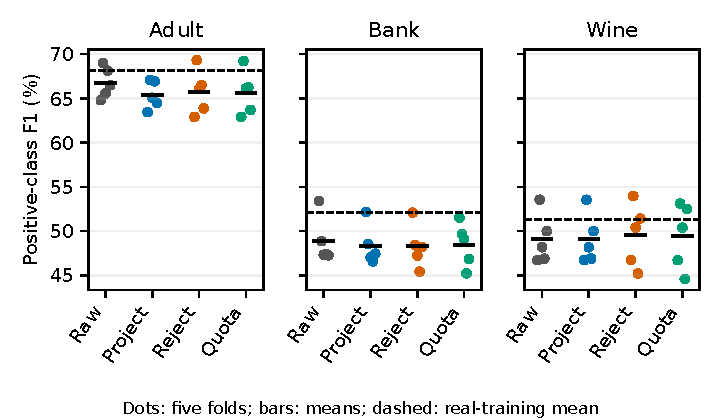
\includegraphics[width=\textwidth]{figures/utility.pdf}
\caption{Conditional-generator utility by fold and processing method.}\label{fig:utility}
\end{figure}
\FloatBarrier

\subsection{Rejection Changes Coverage; Quotas Do Not Recover Utility}
Figure~\ref{fig:selection} shows the mechanism behind the class shift. Across Adult conditional candidate pools, average negative-class acceptance is 22.2\%, compared with 17.5\% for positives. Candidate prevalence averages 25.0\%, while prevalence among all valid candidates averages 20.8\%. Full-pool counts satisfy Eq.~\ref{eq:selection} to numerical precision in all 45 generator/fold pools. This is an accounting identity, not an independent experimental result.

Adult conditional rejection produces an average absolute prevalence drift of 4.36 pp relative to real training data (Table~\ref{tab:audit}), exceeding raw's 0.42 pp. Quotas restore training prevalence exactly here because the training-size release makes the positive count an integer quota. However, quota F1 is 65.6\%, compared with raw 66.8\% and reject 65.7\%. Fixing label counts does not undo feature selection caused by requiring valid rows.

Bank conditional rejection has a smaller but similarly directed imbalance in acceptance: negatives average 90.5\% and positives 80.3\%. Absolute prevalence drift grows from 0.26 pp for raw to 1.30 pp for rejection. Quota F1 averages 48.5\%, between raw 48.9\% and reject 48.3\%; paired quota-minus-reject effects range from $-1.34$ to $+1.87$ pp. These data do not support consistent utility recovery from quotas.

Wine conditional acceptance is nearly equal across classes, 98.2\% versus 98.0\%. Rejection and quotas change F1 modestly on average, and paired quota-minus-reject effects range from $-0.84$ to $+1.05$ pp. This boundary case matters: filtering effects depend on the association between validity and class, not simply on whether a rule is feature-only.

\begin{figure}[!htbp]
\centering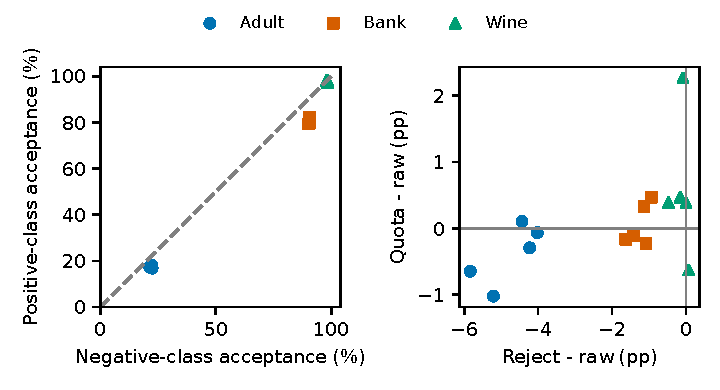
\includegraphics[width=\textwidth]{figures/selection.pdf}
\caption{Conditional-pool acceptance and released prevalence changes by fold.}\label{fig:selection}
\end{figure}
\FloatBarrier

\subsection{Candidate Budget, Fidelity, and Copying}
Table~\ref{tab:audit} combines distinct diagnostics for the conditional generator. Adult ordinary rejection examines 4.74 candidates per released row on average; quotas require 5.75. Bank requires 1.12 and 1.28, and Wine 1.02 and 1.09. All complete within the tenfold pool. Projection's candidate ratio is one, but that does not account for repair computation or imply constant wall-clock cost.

\begin{table}[!htbp]
\caption{Conditional-generator validity, drift, candidate cost, and marginal distance.}\label{tab:audit}
\centering\small
\begin{tabular}{llrrrr}\toprule
Data & Method & Invalid (\%) & Drift (pp) & Candidates/row & Distance \\\midrule
Adult & Raw & 79.4 & 0.42 & 1.00 & 0.012 \\
Adult & Project & 0.0 & 0.42 & 1.00 & 0.012 \\
Adult & Reject & 0.0 & 4.36 & 4.74 & 0.057 \\
Adult & Quota & 0.0 & 0.00 & 5.75 & 0.047 \\
Bank & Raw & 10.7 & 0.26 & 1.00 & 0.012 \\
Bank & Project & 0.0 & 0.26 & 1.00 & 0.012 \\
Bank & Reject & 0.0 & 1.30 & 1.12 & 0.015 \\
Bank & Quota & 0.0 & 0.00 & 1.28 & 0.014 \\
Wine & Raw & 2.1 & 0.83 & 1.00 & 0.037 \\
Wine & Project & 0.0 & 0.83 & 1.00 & 0.037 \\
Wine & Reject & 0.0 & 0.99 & 1.02 & 0.036 \\
Wine & Quota & 0.0 & 0.00 & 1.09 & 0.036 \\
\bottomrule\end{tabular}
\end{table}

Real-training F1 averages 68.2\%, 52.1\%, and 51.3\% on Adult, Bank, and Wine; bootstrap references average 67.6\%, 52.7\%, and 50.9\%. Bootstrap occasionally exceeding the real mean is compatible with finite resampling variation. These references show that most of the conditional generator's utility deficit remains after full constraint satisfaction. Simple processing does not recreate lost joint structure.

Every bootstrap row exactly matches a training row, while none of the 180 generated-method releases contains an exact full-row match. A generator can avoid exact duplicates while retaining sensitive or identifying attributes; we perform no attack-based privacy evaluation. Combining copying rate and utility into a privacy--utility score would make an unsupported inference.
\FloatBarrier

\section{Discussion and Practical Implications}
Validity processing enforces the selected relation, while utility depends on a wider distribution and the learner. Adult projection removes an inconsistent duplicate representation of education, yet F1 decreases for both copulas. This is an observed tradeoff, not a claim that inconsistent records are desirable. Raw release is a diagnostic comparator, and an application may correctly prohibit it regardless of F1.

\paragraph{Use an approval vector.}
A synthetic-data approval pipeline should retain four separate dimensions: \emph{constraint coverage}, \emph{class coverage}, \emph{predictive behavior}, and \emph{candidate cost}. Constraint coverage records which rules were tested and their violation rates; class coverage records prevalence drift and class-conditional acceptance; predictive behavior records task-specific validation metrics; candidate cost records prefix examinations and whether the release completed within its cap. A 100\% validity score supplies evidence only for the tested rules. It must not substitute for the other dimensions or certify privacy.

Set application-specific acceptance criteria for each dimension before inspecting final test outcomes. Retain utility checks on untouched real validation data, including minority-class F1 or recall when these match the intended task. For rejection, record class-conditional acceptance and pool exhaustion alongside overall acceptance: label-blind code can select labels indirectly. If quotas restore prevalence but utility falls below the chosen criterion, the release still fails that utility check; inspect or refit the generator and evaluate a new candidate release. Deployment decisions require a validation partition beyond the final test set used here. This is operational guidance, not a newly evaluated release-selection algorithm.

The shared-pool design reduces one source of noise, but rejection methods do not retain identical records or require equal computation. Their differences describe the full release intervention. Class-balanced training also limits an explanation in which the entire utility effect comes from changed class weights: reweighting counts cannot restore altered within-class associations. A future decomposition could use additional learners, calibration measures, and conditional-distribution tests. The current metrics alone do not establish causal mediation.

The quota result is an empirical counterexample to the sufficiency of matching label counts for the tested learner and generators. It does not prove which within-class association caused a utility change. Privacy evidence also requires a separate assessment: the four-dimensional approval record is a data-quality audit, not a complete release-safety certificate. The contribution is an auditable failure mode and bounded decision guidance rather than a new architecture.

\section{Limitations and Conclusion}
Three small public tasks, one constraint per dataset, one learner, and one generation seed per fold limit generality. Adult is a prefix of complete cases; Bank is the smaller supplied subset; Wine is red only. Random row splits do not establish temporal, institutional, or group transfer. Bank retains call duration, so its task is retrospective classification, not pre-call targeting. Duplicate feature rows across train/test partitions are not deduplicated; wine measurements can repeat. This is not a fairness audit despite reporting positive-class coverage; protected-group disparities require separate investigation.

The copulas use arbitrary alphabetical nominal encodings and empirical inverse marginals. They cannot stand in for CTGAN, diffusion, or constraint-aware neural models. The pool cap never binds, so incomplete-release behavior is tested in code but its deployment frequency is unmeasured. No method provides differential privacy, legal compliance, or attack evaluation. Overlapping training folds provide limited uncertainty evidence.

Within these limits, full tested validity coexists with lower, unchanged, or variably improved minority-class F1. Ordinary rejection can alter class prevalence through unequal acceptance. Quotas fix label counts without guaranteeing utility recovery and can increase the required candidate prefix. A release decision should retain an approval vector of constraint coverage, class coverage, predictive behavior, and candidate cost, with a separate privacy assessment when required. The next step is to extend this paired contract to neural generators, multiple learners, richer constraints, and independent external datasets.

\section*{Declaration on Generative AI}
A generative AI assistant was used to assist study design, implement experimental and analysis code, execute checks, draft and revise text, and prepare figures and references. Numerical results were computed by the accompanying programs rather than generated as text. Human authors must independently verify the scientific reasoning, code, data provenance, citations, results, and manuscript before submission and accept responsibility for them. This draft does not certify that this human review has occurred.

\bibliographystyle{splncs03}
\bibliography{references}
\end{document}
